\documentclass{BHCexam}
\biaoti{~$2013 - 2014$~学年度第一学期期中考试}
\fubiaoti{高二数学试卷}
\usepackage{palatino}
\usepackage{siunitx}%输入度数符号需要的单位宏包
\usepackage{tikz}
\usetikzlibrary{shapes.geometric, arrows}
\tikzstyle{startstop} = [rectangle, rounded corners, minimum width = 1cm, minimum height=0.5cm,text centered, draw = black]
\tikzstyle{io} = [trapezium, trapezium left angle=70, trapezium right angle=110, minimum width=0.5cm, minimum height=0.5cm, text centered, draw=black]
\tikzstyle{process} = [rectangle, minimum width=2cm, minimum height=0.5cm, text centered, draw=black]
\tikzstyle{decision} = [diamond, aspect = 3, text centered, draw=black]
% 箭头形式
\tikzstyle{arrow} = [->,>=latex]

\begin{document}
\maketitle
%\mininotice

\begin{questions}

%选择题
\xuanze
\question 下列叙述错误的是\stk{B}.\\
\fourch{频率是随机的,在试验前不能确定,随着试验次数的增加,频率一般会越来越接近概率}{若随机事件~$A$~发生的概率为~$p(A)$~,则~$0\leq p(A)\leq 1$~}{互斥事件不一定是对立事件,但是对立事件一定是互斥事件}{~$5$~张奖券中有一张有奖,甲先抽,乙后抽,那么乙与甲抽到有奖奖券的可能性相同}
\qs 将十进制数~$89$~化成三进制数的末位数字是\stk{B}.\\
\onech{$1$}{$2$}{$3$}{$0$}
\question 若~$x,y$~满足约束条件~$y\leq x,x+y\leq 1,y\geq -1$~,则~$z=2x+y$~的最大值为\stk{A}.\\
\onech{$3$}{$-3$}{$\dfrac{3}{2}$}{$0$}
\begin{minipage}[b]{0.8\linewidth}
\question 为了了解某地参加计算机水平测试的~$5000$~名学生的成绩,从中抽取了~$200$~名学生的成绩进行统计分析。在这个问题中,~$5000$~名学生成绩的全体是\stk{A}.\\
\twoch{总体}{个体}{从总体中抽取的一个样本}{样本容量}
\question 如图是甲乙两名同学在~$5$~次体育测试的成绩统计茎叶图,若甲乙的平均成绩分别是~$x,y$~,则下列结论正确的是\stk{C}.\\
\twoch{~$x>y$~,乙比甲成绩稳定}{~$x>y$~,甲比乙成绩稳定}{~$x<y$~,乙比甲成绩稳定}{~$x<y$~,甲比乙成绩稳定}
\question 一个数列~$\{a_n \}$~,其中~$a_1=3,a_2=6,a_{n+2}=a_{n+1}-a_n$~,则~$a_5=$~\stk{B}.\\
\onech{$6$}{$-6$}{$-12$}{$-3$}
\question  阅读右图所示的程序框图,运行相应的程序,输出的结果是\stk{D}.\\
\onech{$1$}{$2$}{$3$}{$4$}
\qs 甲乙两人随意入住两间空房,则两人同住一房的概率是\stk{D}.\\
\onech{$\dfrac{1}{3}$}{$\dfrac{2}{3}$}{$\dfrac{1}{4}$}{$\dfrac{1}{2}$}
\qs 在~$\triangle ABC$~中,若~$\dfrac{cosA}{a}=\dfrac{cosB}{b}=\dfrac{sinC}{c}$~,则~$\triangle ABC$~是\stk{B}.\\
\twoch{有一内角为~$30^\circ$~的直角三角形}{等腰三角形}{有一内角为~$30^\circ$~的等腰三角形}{等边三角形}
\end{minipage}
%\hfill
\begin{minipage}[b]{0.2\linewidth}
\begin{flushright}
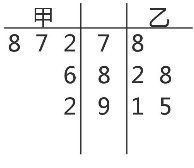
\includegraphics[scale=0.6]{456.png}
\begin{tikzpicture}[node distance=0.2cm]
%定义流程图具体形状
\node[startstop](start){开始};
\node[process, below of = start, yshift = -1cm](in1){$S=2,n=1$};
\node[process, below of = in1, yshift = -1cm](pro1){$S=\frac{1}{1-S}$};
%\node[decision, below of = pro1, yshift = -1cm](dec1){Decision 1 ?};
\node[process, below of = pro1, yshift = -1cm](pro2){$n=n+1$};
\node[decision, below of = pro2, yshift = -1cm](dec1){$S=2$};
\node[io, below of = dec1, yshift = -1cm](out1){输出~$n$~};
\node[startstop, below of = out1, yshift = -1cm](stop){结束};
\coordinate (point1) at (-1cm, -4cm);
%连接具体形状
\draw [arrow] (start) -- (in1);
\draw [arrow] (in1) -- (pro1);
\draw [arrow] (pro1) -- (pro2);
%\draw (dec1) -- node [above] {Y} (point1);
\draw [arrow] (pro2) -- (dec1);
%\draw [arrow] (dec1) -- node [left] {否} (pro1);
\draw [arrow] (dec1) -- node [right] {是} (out1);
\draw [arrow] (out1) -- (stop);
\draw [arrow] (-1.4,-4.8) -- (-2,-4.8) -- (-2,-1.8) -- (0,-1.8);
\node [above right] at (-2,-4.8) {否};
\end{tikzpicture}
\end{flushright}
\end{minipage}

\question 设~$\{a_n \}$~是各项为正数的无穷数列,~$A_i$~是边长~$a_i,a_{i+1}$~为的矩形的面积~$(i=1,2,\cdots)$~,则~$\{A_n \}$~为等比数列的充要条件是\stk{D}.\\
\fourch{~$\{a_n \}$~ 是等比数列}{~$a_1,a_3,\cdots,a_{2n-1},\cdots$~或~$a_2,a_4,\cdots,a_{2n},\cdots$~是等比数列}{~$a_1,a_3,\cdots,a_{2n-1},\cdots$~和~$a_2,a_4,\cdots,a_{2n},\cdots$~均是等比数列}{~$a_1,a_3,\cdots,a_{2n-1},\cdots$~和~$a_2,a_4,\cdots,a_{2n},\cdots$~均是等比数列,且公比相同}

%填空题
\tiankong
\begin{minipage}[b]{0.7\linewidth}
\question 某市高三数学抽样考试中,对~$90$~分以上(含~$90$~分)的成绩进行统计,其频率分布直方图如图所示,若~$130\sim 140$~分数段的人数为~$90$~,则~$90\sim 100$~分数段的人数\stk{810}.\\
\vspace{-15pt}
\question 有一种电子产品,它可以正常使用的概率为~$0.92$~,则它不能正常使用的概率是\stk{0.08}.\\
\end{minipage}
\vspace{-20pt}
\hfill
\begin{minipage}[b]{0.3\linewidth}
\begin{flushright}
\begin{tikzpicture}
\draw[->,>=latex] (0,0) -- (0,3) node[right] {频率/组距};
\draw[->,>=latex] (0,0) -- (4,0) node[above] {分数};
\draw (1,0) -- (1,2.7) -- (1.5,2.7) -- (1.5,0);
\draw (1.5,1.5) -- (2,1.5) -- (2,0);
\draw (2,0.9) -- (2.5,0.9) -- (2.5,0);
\draw (2.5,0.6) -- (3,0.6) -- (3,0);
\draw (3,0.3) -- (3.5,0.3) -- (3.5,0);
\draw[dashed] (0,2.7) -- (1,2.7);
\draw[dashed] (0,1.5) -- (1.5,1.5);
\draw[dashed] (0,0.9) -- (2,0.9);
\draw[dashed] (0,0.6) -- (2.5,0.6);
\draw[dashed] (0,0.3) -- (3,0.3);
\node [below] at (1,0){$90$};
\node [below] at (1.5,0){$100$};
\node [below] at (2,0){$110$};
\node [below] at (2.5,0){$120$};
\node [below] at (3,0){$130$};
\node [below] at (3.5,0){$140$};
\node [left] at (0,2.7){$0.045$};
\node [left] at (0,1.5){$0.025$};
\node [left] at (0,0.9){$0.015$};
\node [left] at (0,0.6){$0.010$};
\node [left] at (0,0.3){$0.005$};
\node [below left] at (0,0){$O$};
\end{tikzpicture}
\end{flushright}
\end{minipage}
\question 设实数~$x,y$~满足~$8^x+2^y=2$~,则~$3x+y$~的最大值是\stk{0}.\\
\vspace{-20pt}
\question 设~$\vartriangle ABC$~的内角~$A,B,C$~所对的边为~$a,b,c$~,且满足~$a cos B -b cos A =\dfrac{3}{5} c$~,则~$\dfrac{tan A }{tan B }=$~\stk{4}\\
\begin{minipage}[b]{0.7\linewidth}
\question 把~$49$~个数排成如图所示的数表,若表中每行的~$7$~个数自左至右依次都成等差数列,每列的~$7$~个数自上而下依次也都成等差数列,且中间的数~$a_{44}=1$~,则表中所有数的和为\stk{49}.\\
\end{minipage}
%\hfill
\begin{minipage}[b]{0.3\linewidth}
\begin{flushright}
\begin{tabular}{|c|c|c|c|}
\hline
$a_{11}$&$a_{12}$&$\cdots$&$a_{17}$\\
\hline
$a_{21}$&$a_{22}$&$\cdots$&$a_{27}$\\
\hline
$\cdots$&$\cdots$&$\cdots$&$\cdots$\\
\hline
$a_{71}$&$a_{72}$&$\cdots$&$a_{77}$\\
\hline

\end{tabular}
\end{flushright}
\end{minipage}

%解答题
\jianda
\question (本小题满分~$12$~分)\\
等比数列~$\{a_n \}$~的前~$n$~项和为~$S_n$~,已知~$S_1,S_2,S_3$~成等差数列.
\begin{parts}
\part 求~$\{a_n \}$~的公比~$q$~;
\part 已知~$a_1-a_3=3$~求~$S_n$~.
\end{parts}
\vspace{8cm}
\question (本小题满分~$12$~分)\\
某车间为了规定工时定额,需要确定加工零件所需花费的时间,为此作了四次实验,得到如下数据:\\
\vspace{-20pt}
\begin{center}
\begin{tabular}{|c|c|c|c|c|}
\hline
~~~零件的个数~$x$~~~(个)&~~~~~~2~~~~~~&~~~~~~3~~~~~~&~~~~~~4~~~~~~&~~~~~~5~~~~~~  \\
\hline
~~~加工的时间~$y$~~~(小时)&~~~~~~2.5~~~~~~&~~~~~~3~~~~~~&~~~~~~4~~~~~~&~~~~~~4.5~~~~~~  \\
\hline
\end{tabular}
\end{center}
\begin{parts}
\part 求出~$y$~关于~$x$~的线性回归方程;
\part 试预测加工~$10$~个零件所需的时间.
\end{parts}
注:可能用到的公式:
\begin{displaymath}
b=\dfrac{\sum\limits_{i=1}^{n} x_iy_i-n \overline{x}\overline{y}}
{\sum\limits_{i=1}^{n} x_i^2-n {\overline{x}}^2},a=\bar{y}-b\bar{x}  
\end{displaymath}
\vspace{8cm}
 \question (本小题满分~$12$~分)\\
 袋中有大小相同的红、黄两种颜色的球各~$1$~个,从中任取~$1$~个,有放回地抽取~$3$~次。求:
 \begin{parts}
\part ~$3$~个全是红球的概率;
\part ~$3$~个颜色全相同的概率.
\end{parts}
\vspace{8cm}
\question (本小题满分~$13$~分)\\
某单位建造一间地面面积为~$12$~平方米的背面靠墙的矩形小房,房子侧面的长度为~$x$~米,房屋正面的造价为每平方米~$400$~元,房屋侧面的造价为每平方米~$150$~元,屋顶和地面的造价费用合计为~$5800$~元,如果墙高为~$3$~米,且不计房屋背面的费用。
\begin{parts}
\part 把房屋总造价~$y$~表示成~$x$~的函数;
\part 当侧面的长度为多少米时,总造价最低?最低总造价是多少?
\end{parts}
\vspace{9cm}
\question (本题满分~$13$~分)\\
$\triangle ABC$中,内角~$A,B,C$~的对边分别为~$a,b,c$~,已知~$b^2=ac,cosB=\dfrac{3}{4}$~.
\begin{parts}
\part 求 ~$\dfrac{1}{tanA}+\dfrac{1}{tanC}$~的值;
\part 设~$\overrightarrow{BA}\cdot \overrightarrow{BC}=\dfrac{3}{2}$~,求~$a+c$~值.
\end{parts}
\vspace{9cm}
\question (本小题满分~$13$~分)\\
对于函数~$f(x)$~,若存在~$x_0\in R$~,使~$f(x_0)=x_0$~成立,则称~$x_0$~为~$f(x)$~的“滞点”.已知函数~$f(x)=\dfrac{x^2}{2x-2}$~.
\begin{parts}
\part 试问~$f(x)$~有无“滞点”?若有求之,否则说明理由;
\part 已知数列~$\{a_n \}$~的各项均为负数,且满足~$4S_n\cdot f(\dfrac{1}{a_n})=1$~,求数列~$a_n$~的通项公式;
\part 已知~$b_n=a_n\cdot 2^n$~,求~$\{b_n \}$~的前项和~$T_n$~.
\end{parts}
\end{questions}
\end{document}
